\section{Evaluation}
\label{sec:eval}

We conducted a comprehensive evaluation to validate our claims. We designed our experiments to answer four key questions: 
\begin {enumerate}
 \item What is the processing overhead of our pipeline's components and how does it scale?
 \item What is the fundamental safety benefit of using an edge-assisted system? 
 \item What is the root cause of the latency-induced failures we observe?
 \item How effectively does our proposed self-beacon anchoring mechanism mitigate these issues?
\end{enumerate}

\subsection{Methodology}

\subsubsection{Experimental Setup and Scenarios}
All experiments were performed on a high-performance workstation equipped with an Intel i9-14900k CPU, 192 GB of DDR5 RAM, and an NVIDIA RTX 4080 Super GPU. We use the \ecav~\cite{eCAV} simulation platform, an open-source framework designed for scalable, edge-assisted CAV simulation built upon CARLA~\cite{dosovitskiy_carla_nodate}. 
We configure the CARLA simulator to run in a synchronous, discrete-time mode with a fixed time step, $\Delta t = 50$~ms, ensuring deterministic and repeatable results. Our evaluation focuses on two high-risk, occlusion-heavy scenarios derived from the NHTSA pre-crash typology (PCT)~\cite{NHTSA_Typology}: 

%\ad{How can we cite eCAV? Otherwise, we can say that we built it, and also mention we'll open-source it? Cited via open source}

\begin{enumerate}
    \item \textbf{Occluded Left Turn (Fig.~\ref{fig:scenario_left_turn}):} An ego vehicle attempts a left turn at an unsignalized intersection while its view of oncoming traffic is obstructed. The NHTSA PCT code of this scenario is C-Left-Turn-Across-Path/Opposite-Direction (LTAP/OD), a common intersection conflict. 
    \item \textbf{Blind Overtake (Fig.~\ref{fig:scenario_overtake}):} An ego vehicle attempts to overtake a stopped firetruck, with its view of a faster-approaching car in the adjacent lane being blocked. The NHTSA of this scenario is B-Straight-Crossing-Path (SCP), which tests the system's ability to handle lateral traffic.
\end{enumerate}


\begin{figure}[h]
    \centering
    % Placeholder for the scenario diagram.
    \includegraphics[trim={5cm 5cm 0cm 0cm}, 
        clip,width=\columnwidth]{figures/occluded_left_turn.png}
    \caption{The Occluded Left-Turn Scenario involving two moving vehicles. The ego vehicle (blue) takes a blind left turn, intersecting with the white vehicle's trajectory. The overlaid blue tracks show the chronological progression of the single ego vehicle as it executes the turn. LTAP/OD Pre Crash Typology Code. %\KR{@Tyler: add more text to the caption so that it is clear that what is shown is the track of the ego vehicle in blue doing the left turn.  One could easily mistake there are 5 distinct cars in the picture shown.}
    }
    \label{fig:scenario_left_turn}
\end{figure}


\begin{figure}[h]
    \centering
    % Placeholder for the scenario diagram.
    \includegraphics[width=\columnwidth]{figures/blind_overtake_2.png}
    \caption{The Blind Overtake Scenario. The ego vehicle initiates an overtake of a large stopped vehicle while its view of oncoming traffic (white vehicle) is obstructed. SCP Overtake Pre Crash Typology Code.}
    \label{fig:scenario_overtake}
\end{figure}

\begin{figure*}[t]
    \centering
\captionsetup[subfigure]{skip=-15pt}
    % --- SUBFIGURE (a) ---
    \begin{subfigure}[b]{0.24\textwidth}
        \centering
        \includegraphics[width=\linewidth]{figures/box_totals.png}
        \caption{Overall Latency Breakdown.}
        \label{fig:box_totals}
    \end{subfigure}\hfill % NO blank line after this
    % --- SUBFIGURE (b) ---
    \begin{subfigure}[b]{0.24\textwidth}
        \centering
        \includegraphics[width=\linewidth]{figures/box_vehicle.png}
        \caption{Vehicle-Side Components.}
        \label{fig:box_vehicle}
    \end{subfigure}\hfill % NO blank line after this
    % --- SUBFIGURE (c) ---
    \begin{subfigure}[b]{0.24\textwidth}
        \centering
        \includegraphics[width=\linewidth]{figures/box_edge.png}
        \caption{Edge-Side Components.}
        \label{fig:box_edge}
    \end{subfigure}\hfill % NO blank line after this
    % --- SUBFIGURE (d) ---
    \begin{subfigure}[b]{0.24\textwidth}
        \centering
        \includegraphics[width=\linewidth]{figures/edge_latency_compare_box.png}
        \caption{Edge Compute Cost.}
        \label{fig:edge_compute_cost}
    \end{subfigure}
    % All subfigures are now on a "single line" in the code.
    %\vspace{-3mm}
    \caption{Processing-time breakdown of the end-to-end perception pipeline. (a) End-to-end latency is dominated by network and on-vehicle processing. (b) On-vehicle, perception (YOLOv5) is the main contributor. (c) On-edge, the tracker (AB3DMOT) is the main contributor. (d) The overhead of our proposed Beacon-Edge protocol is negligible ($\sim$0.2ms).}
    \label{fig:latency_breakdown_combined}
\end{figure*}



\begin{figure}[h]
    \centering
    \includegraphics[width=\columnwidth]{figures/AB3DMOT_scalaiblity.png}
    \caption{Edge tracker scalability. Latency grows quadratically with the number of objects, becoming a significant contributor of the end-to-end pipeline processing time in dense scenarios.}
    \label{fig:scalability}
\end{figure}


\subsubsection{End-to-End Latency Models}
\label{sec:e2e_lat_model}
To comprehensively characterize the safety envelope, we employ two distinct latency models in our evaluation.

First, to clearly isolate the system's core failure modes under deterministic conditions, our primary experiments (Sections~\ref{sec:sys_perf} through \ref{sec:hazard_dynamics}) model the total end-to-end latency as a fixed data staleness. This is implemented by processing data from a past time step $k$ to simulate a precise, repeatable total delay of $L = k \cdot \Delta t$.

Second, to validate our findings against realistic network conditions, we developed a high-fidelity, component-based hybrid latency model. This model, derived from our budget in Table~I, calculates the total end-to-end latency at each simulation step by summing the individual processing and networking delays. We ground our simulation in empirical data by driving the networking components with real-world measurements. The highly variable C-V2X radio link is modeled using a latency trace from the public SEE-V2X dataset~\cite{seev2x}. For the RSU-to-Edge backhaul, we use a trace-informed stochastic model, parameterizing a log-normal distribution to match the median and 99th-percentile RTT reported in the 5G-MOBIX field trials~\cite{5gMobix2023}. These variable components are then additively combined with other system delays, such as onboard perception and edge compute times. This high fidelity model is used exclusively for our network jitter analysis in Section~\ref{sec:jitter_results} and in Table \ref{tab:loss_sensitivity}.


\begin{table}[t]
\footnotesize
\centering
\caption{End-to-end latency components for a MEC deployment (Vehicle→Edge→Vehicle). All stages aligned to a 50 ms control tick.}
\label{tab:latency_mec}
\begin{tabularx}{\columnwidth}{@{}X c@{}}
\toprule
\textbf{Stage} & \textbf{Latency (ms)} \\
\midrule
1. Sensor → On‐board Perception & 20–50 \\
2. Control‐Tick Wait & 0–50 \\
3. Packaging / Serialization & $\sim$5 \\
4. Radio Uplink (C‐V2X PC5 Mode 4)~\cite{Jeon2018ReselectionLookahead} & 30–80 \\
5. Backhaul to MEC Rack~\cite{MECLatency} & $\sim$5~\cite{MECLatency} \\
6. Edge Compute (fusion + tracking + pred) & 20–30 \\
7. Backhaul from MEC~\cite{MECLatency} & $\sim$5~\cite{MECLatency} \\
8. Radio Downlink (C‐V2X PC5 Mode 4)~\cite{Jeon2018ReselectionLookahead} & 30–80~\cite{Jeon2018ReselectionLookahead} \\
9. Control‐Tick Wait & 0–50 \\
10. Planner → Actuation & 5–10 \\
\midrule
\textbf{Total Best‐Case} & $\approx$110 \\
\textbf{Total Average} & $\approx$190 \\
\bottomrule
\end{tabularx}
\vspace{3mm}
\end{table}


\subsection{Results and Analysis}

\subsubsection{System Performance and Scalability}
\label{sec:sys_perf}
We first analyze the computational cost of our pipeline's components. Figure~\ref{fig:latency_breakdown_combined}(a) shows that vehicle-side perception is the most computationally intensive part of the pipeline, with a median processing time of $\sim$25~ms. The entire edge-side intelligence pipeline, by contrast, is an order of magnitude faster in low-density scenarios. Figures~\ref{fig:latency_breakdown_combined}(b) and (c) further show that vehicle-side latency is dominated by the YOLOv5 detector, while edge-side latency is dominated by the AB3DMOT tracker. Critically, Figure~\ref{fig:edge_compute_cost} shows that the overhead of our self-beaconing logic is negligible (a median increase of only 0.2~ms compared to baseline), proving that its substantial safety benefits come at a small compute cost.

However, this experiment focuses on a relatively sparse scene; for denser urban deployments, scalability is a practical concern for both the vehicle and the edge. We benchmarked the AB3DMOT tracker's performance as a function of the number of concurrent objects (Figure~\ref{fig:scalability}). As the Naive and Beacon variants have indistinguishable scalability performance, we show a single line. The tracker latency grows quadratically ($O(N^2)$), reaching 35~ms at 200 objects. In addition, the on-vehicle perception latency also scales with scene complexity; while our microbenchmarks show 25 ms in a sparse scene, this latency would also increase with a higher number of objects to detect and track. These scalability results demonstrate that for dense deployments, the total compute time from both the vehicle and the edge becomes a significant factor that can consume a large portion of the safety envelope, shrinking the available budget for network communication.

%\smallskip\noindent\textbf{Compute headroom.}\,
%A four-frame CUDA stream fusion accelerates the AB3DMOT association kernel from 330 Hz to 1.3 kHz on an RTX 3080—a \mbox{$4\times$} speedup that suggests ample compute margin for dense, city-scale deployments.

\subsubsection{Bandwidth Cost}

\begin{table}[t]
\footnotesize
\centering
\caption{Per-vehicle uplink budget at \textbf{20 Hz}.
         Statistics computed over all frames in both scenarios
         (\(n\!=\!2{,}000\)); each vehicle sent at most 10 boxes per frame.}
\label{tab:bandwidth}
\begin{tabularx}{\linewidth}{@{}lccc@{}}
\toprule
\textbf{Msg type} & \textbf{Avg.\ size (B)} & \textbf{p95 (B)} & \textbf{KB/s}\\
\midrule
Self-beacon (fixed)        & 96   & 96    & 1.88 \\
3-D bbox list ($\leq$10 boxes)  & 4,130 & 4,720 & 8.06 \\
\midrule
\textbf{Total}             & —    & —     & \textbf{9.94} \\
\bottomrule
\end{tabularx}
%\vspace{-0.6em}
\end{table}

Each vehicle transmits its data to the nearest edge over a C-V2X link. The uplink payload consists of two parts: (1) a 96\,B self-beacon, whose binary layout is fixed, and (2) a variable-length list of 3-D bounding boxes. Across all 2,000 evaluation frames, no vehicle ever uploaded more than ten boxes; the empirical mean was seven. Table~\ref{tab:bandwidth} summarizes the resulting bandwidth demand at the required 20\,Hz publish rate. Even in the worst case, the total uplink is only \(\approx 9.9\;\mathrm{KB/s}\) per vehicle. This bandwidth demand is significantly lower than early-fusion systems like EMP that stream raw LiDAR (\(\sim\!3.7\;\mathrm{MB/s}\) per vehicle~\cite{EMP, Autocast, harbor}). It is also one to two orders of magnitude lower than systems that transmit intermediate features, such as F-Cooper (\(\sim\!200-900\;\mathrm{KB/s}\)~\cite{fcooper}) or V2X-ViT (\(\sim\!1.3\;\mathrm{MB/s}\)~\cite{v2xvit2022}).

\subsubsection{Characterizing the Edge Safety Envelope and its Root Cause}

We now analyze the impact of the end-to-end edge-assisted perception pipeline's latency on safety. For this analysis, we define our primary metric, Scenario Success Rate, as the percentage of simulation runs where the ego-vehicle reaches its destination without incurring a collision, a deadlock, or a false-braking event attributable to the self-ghosting artifact.

%\ad{Must define the metric of "scenario success rate" first. Tyler: Fixed} 
Figure~\ref{fig:success_vs_latency} shows the success rate for our two evaluated scenarios as we sweep that delay. 
Recall that the end-to-end delay includes three main components: on-vehicle perception, vehicle-edge communication (two ways), and on-edge computation time.
In both scenarios, the \textbf{Naive-Edge} system's performance exhibits a sharp success rate drop once latency exceeds a certain threshold ($\sim$150~ms in the Occluded Left Turn scenario), defining the boundary of its safety envelope. Our \textbf{Beacon-Edge} system, however, remains 100\% successful until much higher latencies ($\sim$300--400~ms), demonstrating a substantially expanded safety envelope. The physical reason for this cliff is motion-induced position error ($\Delta x = v \cdot \Delta t$), which eventually exceeds the tracker's gating radius and leads to the ``self-ghosting'' artifact where a stale track is duplicated.
These results indicate that Beacon-Edge is significantly more versatile and resilient, allowing slower or less reliable networks, or supporting longer computations on vehicles and on the edge.

\begin{figure*}[t]
    \centering
    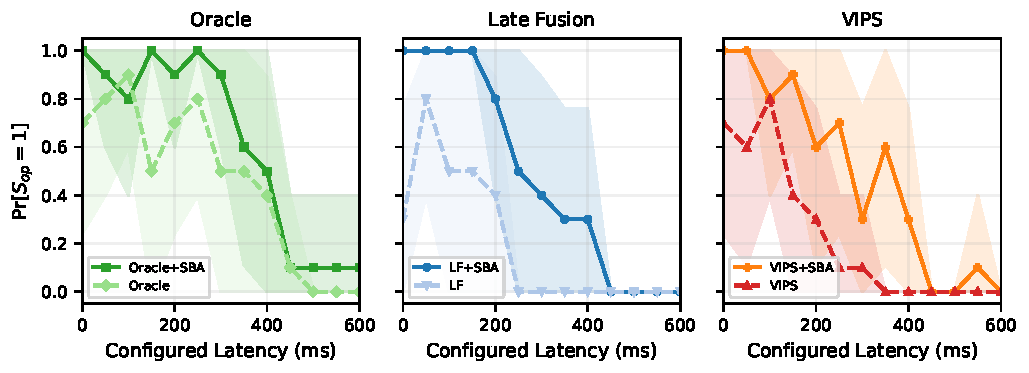
\includegraphics[width=\textwidth]{figures/success_vs_latency.pdf}
    \caption{Operational success $P(S_{op})$ vs.\ configured latency for each manager, with SBA on and off on the same axes. Late Fusion and VIPS exhibit a sharp safety cliff around ${\sim}100\text{--}150\,\mathrm{ms}$. Oracle maintains high $S_{op}$ until the physics-limited boundary at ${\sim}300\text{--}400\,\mathrm{ms}$. With SBA, the multi-source stacks track the Oracle curve.}
    \label{fig:success_vs_latency}
\end{figure*}


\begin{figure*}[t]
    \centering
    \subfloat[Occluded Left Turn scenario.]{
    \includegraphics[width=\columnwidth]{figures/olt_false_braking_event.png}
    }
    \subfloat[Blind Overtake scenario.]{
    \includegraphics[width=\columnwidth]{figures/overtake_false_braking_events.png}
    }
    \caption{Efficacy of Self-Beacon Anchoring: False-Braking Events vs. end-to-end latency of the edge-assisted perception pipeline for our two evaluated scenarios. Beacon-Edge: 0 across all latencies. Naive-Edge spikes after ~100 ms.}
    \label{fig:false_braking_results}
\end{figure*}


\begin{figure*}[t]
    \centering
    \subfloat[Occluded Left Turn scenario.]{
    \includegraphics[width=\columnwidth]{figures/olt_ttc_vs_latency.png}
    }
    \subfloat[Blind Overtake scenario.]{
    \includegraphics[width=\columnwidth]{figures/overtake_ttc_vs_latency.png}
    }
    \vspace{-3mm}
    \caption{Average Time-to-Collision (TTC) vs. end-to-end latency of the edge-assisted perception pipeline for our two evaluated scenarios. The Beacon-Edge system consistently provides a larger safety margin (higher TTC) across latencies.}
    \label{fig:ttc_vs_latency}
\end{figure*}

\subsubsection{Efficacy of Self-Beacon Anchoring}
To provide direct evidence of the self-ghosting problem and the efficacy of our solution, we measured the rate of false-braking events. As shown in Figure~\ref{fig:false_braking_results}, the Naive-Edge system experiences a dramatic spike in hazardous, unnecessary braking maneuvers as latency increases beyond 100~ms. In stark contrast, our Beacon-Edge protocol completely eliminates this failure mode across all tested latencies in both scenarios by successfully solving the targeted state-consistency problem.

To further quantify the safety margin, we analyze the \textbf{Time-to-Collision (TTC)}, defined as the time it would take for two vehicles to collide if they continued at their current speed and orientation. Figure~\ref{fig:ttc_vs_latency} shows the TTC distribution for the subset of runs that did not result in a collision. For the Naive-Edge system, even in the few instances where it succeeds at high latency, it does so with a dangerously low TTC. Our \textbf{Beacon-Edge} system consistently maintains a much higher and safer median TTC, reinforcing that our architectural improvements not only increase the success rate but also improve the quality and safety margin of those successes.

\begin{table}[t]
\footnotesize
\centering
\caption{Anchoring success rate under the hybrid 190 ms latency model
(20 runs).}
\label{tab:loss_sensitivity}
\begin{tabularx}{\linewidth}{@{}l*{5}{>{\centering\arraybackslash}X}@{}}
\toprule
\textbf{PC5 loss (\%)} & 0 & 5 & 10 & 12 & 15 \\ \midrule
Success rate (\%)      & 100 & 100 & 100 & 80 & 5 \\ \bottomrule
\end{tabularx}
%\vspace{-0.5em}
\end{table}

As Table~\ref{tab:loss_sensitivity} shows, a 20-run sweep indicates anchoring offers at least a $2\times$ reliability margin over real RSU links ($\leq 5\%$ loss in SEE-V2X \cite{seev2x}). This aligns with the latency sweep where anchoring also maintained $100\%$ success within the 300 ms envelope.

%\ad{How does this work for Naive? I thought there are no successful runs beyond 200ms for occluded turn and beyond 400ms for blind overtake.}
%\ad{Again, we should define the TTC metric. Is it "the time it would take for vehicles to collide if they continued at their current speed and orientation"?}




\subsubsection{Impact of Hazard Vehicle Dynamics}
\label{sec:hazard_dynamics}
%\ad{what is axis 3? Was there a 1 and 2? Tyler: removed}
Finally, we analyze how the different system configurations handle increasing dynamic difficulty (i.e., ``aggressive'' driving behaviors) in the Occluded Left-Turn scenario. For this experiment, we vary the independent variable that most directly impacts safety: the speed of the occluded, oncoming vehicle. While the ego vehicle's time to ``peek'' around the obstruction is constant, a higher speed for the hazard vehicle dramatically reduces the available time to react and stop, making the scenario more challenging. We test all three configurations, with the end-to-end edge-assisted perception latency fixed at a challenging 200~ms value.

The results, shown in Figure~\ref{fig:olt_speed_cliff}, highlight the clear safety hierarchy of the systems.
\begin{itemize}
    \item The \textbf{Local-Only} system fails almost immediately. Once the oncoming vehicle's speed exceeds a mere 10~km/h, the ego-vehicle, upon seeing the hazard, no longer has the physical braking distance required to avoid a collision.

    \item The \textbf{Naive-Edge} system leverages its beyond-line-of-sight awareness to perform better, but its performance collapses at moderate speeds. The combination of a faster-moving object and the 200~ms latency is sufficient to trigger the ``self-ghosting'' false braking events, leading to erratic behavior and a high collision rate. 

    \item Our \textbf{Beacon-Edge} system, however, remains robust and successful across the full range of tested speeds. By having early, reliable awareness of the occluded vehicle and being immune to the self-ghosting artifact, it can accurately predict the hazard's trajectory and safely yield, demonstrating a vastly superior operational domain.
\end{itemize}

\begin{figure}[t]
    \centering
    \includegraphics[width=\columnwidth]{figures/critical_speed_cliff.png}
    \caption{Impact of Hazard Dynamics in Occluded Left-Turn Scenario (at 200 ms latency) evaluated as Success Rate vs. Occluded Vehicle Speed. Our Beacon-Edge system remains safe at high speeds until around 40 km/h, while the Naive-Edge and Local-Only systems fail as the scenario's difficulty increases.}
    \label{fig:olt_speed_cliff}
\end{figure}

\subsubsection{Robustness to Trace-Driven Network Jitter}
\label{sec:jitter_results}
We validate our findings using the high-fidelity hybrid latency model described in Section \ref{sec:e2e_lat_model}. The results for 10 trials per configuration are presented in Figure~\ref{fig:jitter_results}. The points represent the mean success rate against the empirically measured mean latency, with error bars showing the standard error of the mean (vertical) and the standard deviation of the measured latency (horizontal).

The results strongly reinforce our deterministic findings. The Naive-Edge system's performance still collapses rapidly around the 150\,ms mark, while Beacon-Edge maintains a high success rate to beyond 300\,ms. This experiment validates that the safety benefits of Self-Beacon Anchoring persist in a non-deterministic environment that reflects the specific statistical patterns of real-world V2X and 5G edge networks


\input{floats/float-olt-jitter}


%\ad{Rather than critical speed cliff, we need to detrmine the reaction window. How much time do we have to make a decision? Time to detection of a collision.}

%\kishore{Only AVs are capable of doing prediction computation, scenario includes AVs and non AVs, the edge provides trajectories of non AVs, if AVs are only doing the omputation. Total amount of work done is N times the number of AVs which at the edge, it's only 1 at the edge. Doing everything on the edge means single point of failure. Run your own calculations, have qualitiative discussion on the pros and cons. Decision making is happening, edge can make decisions. No consideraion for decision making at the edge. Quality of the prediction algorithm is orthogonal. Also incorporate things about why we chose late fusion vs early fusion.}

%\kishore {System architecture should be talking about avs and non avs in the scenario, and how edge asssisted acontrol. For evaluation, we have resetricted to sceanrios wehre there is only 1 av and a bunch of other vehicles and objects taht hte vehicle has to worry about. In discussion, broadening the scope, what is how the envelope comes to play. The comms won't be affected, but the compute latency will get higher, adn more complicated prediction. need to talk qwualitatively about the scalabiltiy in the discussion}